\documentclass[11pt, oneside]{article}   	% use "amsart" instead of "article" for AMSLaTeX format
\usepackage{geometry}                		% See geometry.pdf to learn the layout options. There are lots.
\geometry{letterpaper}                   		% ... or a4paper or a5paper or ... 
%\geometry{landscape}                		% Activate for for rotated page geometry
%\usepackage[parfill]{parskip}    		% Activate to begin paragraphs with an empty line rather than an indent
\usepackage{graphicx}				% Use pdf, png, jpg, or eps§ with pdflatex; use eps in DVI mode
								% TeX will automatically convert eps --> pdf in pdflatex		
\usepackage{amssymb}
\usepackage{longtable}        % for table that can span multiple pages
\usepackage{authblk}          % for author affiliations

\title{Amplicon sequencing (16S and ITS) processing platform}
\author{Thomas Gurry (thomasgurry@gmail.com)}
\author{Claire Duvallet (duvallet@mit.edu)}
\affil{Center for Microbiome Informatics and Therapeutics}

\date{}							% Activate to display a given date or no date

\begin{document}
\maketitle
\tableofcontents
\section{Introduction}
This document describes the process of going from raw 16S or ITS data to processed data (OTU tables, oligotypes, etc.).  This is orchestrated by the script {\tt raw2otu.py}.  The platform is designed in such a manner that the user interfaces with a single script, {\tt Master.py}, which takes as input the path to the folder containing the dataset.  Each dataset folder must contain a machine-readable text file, called a summary file, which gives instructions to {\tt Master.py}.  The format of these summary files, and all files required for 16S or ITS processing, are described in the section below.

\section{Preparing your dataset for processing}
\subsection{Raw data files}
The first step to process your data is to understand what raw data you have.
Do you have FASTQ or FASTA data? Are your sequences already de-multiplexed with
one file per sample, or will you need to split sequences by barcodes?
Do you have unmerged forward and reverse reads that you'll need to merge?
Are the primers still in the sequences? Are they already all trimmed to a certain
length? Every sequencing center provides a different kind of "raw data", so
make sure you know what you're starting with! The pipeline takes many different
kinds of inputs and can perform many different processing steps, so it's
important to know what you'll be needing.

\subsection{Summary file}
This file, named {\tt summary\_file.txt}, is a machine-readable, \textbf{tab-delimited} 
file that must accompany any dataset directory when uploaded to the cloud. 
It orchestrates all processing that will happen, and is where you specify each
of your processing requests. It should be found in the highest directory level 
for the dataset directory in the S3 bucket.  It is a text file with descriptors 
for the data and paths to all relevant datafiles within the directory.  
It can include a True or False flag for whether any associated raw 16S/ITS data has 
already been processed. It is case-sensitive.

The order in which items are listed between the lines {\tt \#16S\_start} and {\tt \#16S\_end} 
(for 16S) and between lines {\tt \#ITS\_start} and {\tt \#ITS\_end} (for ITS) does not matter.  

Note that any white space in the summary file should correspond to a single tab character.

\subsection{Summary file format and options}

The first line in your summary file should be:

\begin{verbatim}
DATASET_ID	myDataset
\end{verbatim}

16S and ITS processing parameters are specified by attributes placed
on separate lines between \texttt{\#16S\_start} and \texttt{\#16S\_end}
and/or \texttt{\#ITS\_start} and \texttt{\#ITS\_end}. All white spaces in the
summary file should be tabs.

Required attributes are: \texttt{PRIMERS\_FILE}, \texttt{BARCODES\_MAP}, \texttt{PROCESSED} and
one of: \texttt{RAW\_FASTQ\_FILES}, \texttt{RAW\_FASTA\_FILE}, and \texttt{RAW\_FASTA\_FILES}.

For processing to occur,  \texttt{PROCESSED} should be \texttt{False} (case-sensitive).

The following section will go through all available summary file attributes, and
are summarized in Appendix \ref{sec:summarytable}.
These options are presented in roughly the same order as they
are processed.

\subsubsection{Input file(s)}

The pipeline takes as input many kinds of raw data:

\begin{itemize}
	\item one FASTQ file. This file should contain all sequences for all of your 
	samples. Sequences may still contain barcodes, or they can have had barcodes
	removed and FASTQ headers replaced with sample identifiers.
	\item multiple FASTQ files. Each of these files should contain sequences for
	one sample only. 
	\item one FASTA file. This file should contain all sequences for all of your 
	samples, and should have a sample identifier in the FASTA header line.
	\item multiple FASTA files. Each of these files should contain sequences for 
	one sample only.
\end{itemize}

You can specify the type of file input by using the , 
\texttt{RAW\_FASTQ\_FILES}, \texttt{RAW\_FASTA\_FILE}, and \texttt{RAW\_FASTA\_FILES} attributes.

If you have one sequence file, \texttt{RAW\_FASTQ\_FILE} or \texttt{RAW\_FASTA\_FILE}
should refer to the FASTQ/A file name. If you have multiple sequence files, 
\texttt{RAW\_FASTQ\_FILES} or \texttt{RAW\_FASTA\_FILES} should refer to 
a text file that relates each FASTQ/A file to its sample identifier.
This text file is tab-delimited with the FASTQ/A file name in the first column
and the corresponding sample ID in the second column. This text file should
not contain a header.

Note that all file paths provided should be 
\textit{relative to the summary file directory}. If your FASTQ to sample ID
file map is in a subdirectory called \texttt{filemaps/} and your
sequence files are in a subdirectory called \texttt{datafiles/}, then 
\texttt{RAW\_FASTQ\_FILES} would be \texttt{filemaps/fastq\_filemap.txt},
and \texttt{fastq\_filemap.txt} would include \texttt{filemaps/file1.fastq}, etc.

\subsubsection{Merging}

If you have unmerged paired-end reads, you can merge them by setting 
\texttt{MERGE\_PAIRS} to \texttt{True} (case sensitive). Merging can be
performed in both the case where your reads are not de-multiplexed (i.e.
you have one file with \textit{all} of your forward reads for all of your
samples, and one file with all of the reverse reads) and when they are
(i.e. you have two files per sample: one with the forward reads and one with
the reverse reads). 

If you need to merge reads, you also need to specify the file name suffixes
for both the forward and reverse read files. These are specified in
\texttt{FWD\_SUFFIX} and \texttt{REV\_SUFFIX} and default to \texttt{\_R1.fastq}
and \texttt{\_R2.fastq}, respectively. If you have more complicated file names,
either rename them to have consistent suffixes, or talk to Claire to see if you
can incorporate more complicated regex matching into the code.

Note that the files specified either in \texttt{RAW\_FASTQ\_FILE} or in the
\texttt{fastq\_filemap.txt} (specified in \texttt{RAW\_FASTQ\_FILES}) should refer
to the FASTQ files containing the forward reads.

See Case 4 in Section \ref{sec:case4} for an example.

\subsubsection{De-multiplexing}

If your FASTQ file still contains the barcodes in the sequences, you
will need to include \texttt{BARCODES\_MAP} and \texttt{BARCODES\_MODE}
in your summary file. \textbf{**Note that \texttt{BARCODES\_MAP} is a 
required attribute.} If you do not need to de-multiplex your sequences,
\texttt{BARCODES\_MAP} should be \texttt{None} (case-sensitive).

\texttt{BARCODES\_MAP} refers to a tab-delimited file which has the
sample identifiers in the first column and the corresponding barcode sequence
in the second column. This file does not have a header. 

You must also specify a \texttt{BARCODES\_MODE}, which specifies where the
barcodes are to found in the FASTQ file. If the barcodes are still in the
sequences, \texttt{BARCODES\_MODE} should be 2. If the barcodes are in
the FASTQ sequence header, \texttt{BARCODES\_MODE} should be 1.

See Case 1 in Section \ref{sec:case1} for an example.

Sometimes, the 'raw' data has already had primers and barcodes removed 
but still has all samples in the same FASTQ file. In this case, \texttt{BARCODES\_MAP} 
should be \texttt{None} and the sample IDs must be listed in the sequence header 
lines of the FASTQ file. If there is text other than the sample ID
in the header, you need to specify the first non-sample ID character
in \texttt{BARCODES\_SEPARATOR}. For example, sequences in these kinds of
files are often labeled like:

\begin{verbatim}
@sample1_seq1
...<rest of fastq record>
@sample1_seq2
...<rest of fastq record>
@sample2@_seq1
...<rest of fastq record>
@sample3_seq1
...<rest of fastq record>
@sample2_seq2
...<rest of fastq record>
\end{verbatim}

In this case, the barcodes separator would be an underscore (\texttt{\_}), which is the default.

\subsubsection{Primer trimming}

If you need to remove primers from your sequences, you can specify 
\texttt{PRIMERS\_FILE}, a text file with your primer sequences.
\textbf{**Note that \texttt{PRIMERS\_FILE} is a 
required attribute.} If you do not need to remove primers from your sequences,
\texttt{PRIMERS\_FILE} should be \texttt{None} (case sensitive).

The pipeline does not currently remove reverse primers. If your sequences
still contain reverse primers, you can remove them yourself or trim your 
sequences to a length shorter than the start of your reverse primer.

\subsubsection{Quality filtering}

There are two ways to quality filter your sequences.
One is based on the number of expected errors in your sequence, and the other
truncates reads after a certain quality is encountered. You can learn more
about these approaches by reading the USEARCH documentation:
http://www.drive5.com/usearch/manual/readqualfiltering.html

To truncate reads after a base with a certain quality is encountered, use the
\texttt{QUALITY\_TRIM} option. A default value that is often used is 25.
This step is performed \textit{before} length trimming. 

To discard reads based on their number of expected errors, use the 
\texttt{MAX\_ERRORS} option. A default value that is often used is 2 (i.e.
reads with more than 2 expected errors are discarded). This step is
performed \textit{after} length trimming

If nothing is specified, the pipeline defaults to \texttt{QUALITY\_TRIM} of 25.
If both \texttt{MAX\_ERRORS} and \texttt{QUALITY\_TRIM} are specified,
quality filtering by truncation is performed (i.e. \texttt{MAX\_ERRORS} is
ignored).

You may also need to specify the encoding of the quality scores. \texttt{ASCII\_ENCODING} 
can be either \texttt{ASCII\_BASE\_33} (default) or \texttt{ASCII\_BASE\_64}.
You can check the encoding of your file using usearch: \texttt{usearch -fastq\_chars yourFASTQfile.fastq}

\subsubsection{Length trimming}

By default, the pipeline trims all reads to 101 base pairs before
dereplication and clustering. You can specify a different length by
using \texttt{TRIM\_LENGTH}. Any reads which are shorter than the specified
length are discarded.

\subsubsection{Dereplication}

In the dereplication step, unique sequences are identified and the
samples from which they came are tracked (sometimes referred to as 
``provenancing''). By default, unique sequences which are present fewer
than 10 times in the entire dataset are discarded. If you want to change
this number, specify it with \texttt{MIN\_COUNT}.  (e.g. if \texttt{MIN\_COUNT}
is 2, only singleton sequences are discarded).

\subsubsection{OTU clustering}

You can specify the similarity used to define OTUs in the \texttt{OTU\_SIMILARITY}
attribute. The default value is 97, corresponding to 97\% OTUs.

By default, the pipeline clusters OTUs using both \textit{de novo} and closed-reference
approaches. If you specify an OTU similarity that does not have a corresponding
Green Genes reference file, closed-reference clustering will not be performed. 
OTU similarities supported by Green Genes closed-reference mapping are: 61, 64, 67, 70, 73, 76, 79, 82, 85, 88, 91, 94, 97, and 99\%. 
The database files used for this mapping can be found in \texttt{/home/ubuntu/databases/gg\_13\_5\_otus/rep\_set\_latin/}.

The pipeline assigns taxonomies to \textit{de novo} OTUs using the naive-Bayes RDP
classifier. By default, the confidence cutoff is 0.5. You can specify a different
value with the \texttt{RDP\_CUTOFF} attribute.

\subsection{Sample summary files}

\subsubsection{Case 1: raw FASTQ file of 16S sequences, still includes primers and barcodes}\label{sec:case1}

The simplest case is if you have the following files: a raw FASTQ file; a file specifying the map between barcode sequences and IDs; and a file specifying the primers used.  Your summary file would look something like this:

\begin{verbatim}
DATASET_ID	myDataset

#16S_start
RAW_FASTQ_FILE      myData.fastq
ASCII_ENCODING      ASCII_BASE_33
PRIMERS_FILE        primers.txt
BARCODES_MAP        barcodes_map.txt
BARCODES_MODE       2
METADATA_FILE       metadata.txt
PROCESSED           False
#16S_end
\end{verbatim}
Note that you \textbf{must} also specify the place where barcodes are to be found, i.e. either in the "$>$" sequence ID lines (mode 1) or in the sequences themselves (mode 2).  The {\tt PROCESSED} flag tells the processing instance that the dataset needs to be processed into OTU tables.

Your {\tt barcodes\_map.txt} file would look something like this:

\begin{verbatim}
S1      ATCGCTAGTA
S2      TCGCTATATA
S3      TCTACAGCGT
S4      CGTACTCAGT
\end{verbatim}

\subsubsection{Case 2: raw FASTQ file of ITS sequences, primers and barcodes have been removed}
In the case where the 'raw' data has already had primers and barcodes removed (but is not yet de-multiplexed, i.e. all samples are still in the same FASTQ file), the sample IDs must be listed in the sequence ID lines of the FASTQ file.  When the pipeline removes barcodes itself and replaces them with sample IDs, individual sequence reads for a given {\tt sampleID} will be annotated as {\tt sampleID;1, sampleID;2}, etc., where we note here that the {\tt BARCODES\_SEPARATOR} is ';'.  However, in a dataset where the barcodes have previously been removed, you will have to look into the FASTQ file to check the 'separator' character.  Your summary file would look something like this:

\begin{verbatim}
DATASET_ID	myDataset

#ITS_start
RAW_FASTQ_FILE     myData.fastq
ASCII_ENCODING     ASCII_BASE_33
PRIMERS_FILE       None
BARCODES_MAP       None
BARCODES_SEPARATOR ;
METADATA_FILE      metadata.txt
PROCESSED          False
#ITS_end
\end{verbatim}
		
\subsubsection{Case 3: multiple demultiplexed raw FASTQ or FASTA files of 16S sequences, each file corresponding to a single sample}

Sometimes sequencing data are available in a demultiplexed form, where the reads for each sample are split into separate files.  Many datasets in the SRA, for example, are available in this form.  In this case, you can create a \textbf{two-column, tab-delimited file} where the first column lists the filename and the second column lists the corresponding sample ID.  Note that paths should be relative paths \textit{within the current directory}, e.g. {\tt datafiles/file1.txt} for a folder called {\tt datafiles} within the current directory.  In the summary file, the {\tt RAW\_FASTQ\_FILE} line becomes {\tt RAW\_FASTQ\_FILES} (plural), and instead refers to this filename.  If your files are FASTA rather than FASTQ, simply use {\tt RAW\_FASTA\_FILES} (also plural).  For a filename {\tt fastq\_filemap.txt}, your summary file would look something like this:

\begin{verbatim}
DATASET_ID	myDataset

#16S_start
RAW_FASTQ_FILES     fastq_filemap.txt
ASCII_ENCODING      ASCII_BASE_33
PRIMERS_FILE        primers.txt
METADATA_FILE       metadata.txt
PROCESSED           False
PRIMERS_FILE        None
BARCODES_MAP        None
#16S_end
\end{verbatim}

And your {\tt fastq\_filemap.txt} file would look something like this (note that white spaces in the following example correspond to a single tab character):

\begin{verbatim}
SRR10001.fastq	S1
SRR10002.fastq	S2
SRR10003.fastq	S3
SRR10004.fastq	S4
\end{verbatim}

\subsubsection{Case 4: multiple demultiplexed raw paired-end FASTQ files of 16S sequences which need merging}\label{sec:case4}
If your 16S FASTQ files are split into forward and reverse paired-end reads, the pipeline can merge them for you. Specify {\tt MERGE\_PAIRS} in the summary file, and also include the filename suffixes corresponding to forward and reverse reads. If your forward read fastq files were named {\tt sampleID\_L001\_R1.fastq} and your reverse read fastq files were named {\tt sampleID\_L001\_R2.fastq}, your summary file would look something like this:

\begin{verbatim}
DATASET_ID	myDataset

#16S_start
RAW_FASTQ_FILES fastq_filemap.txt
PRIMERS_FILE    None
BARCODES_MAP    None
MERGE_PAIRS	    True
FWD_SUFFIX      _L001_R1.fastq
REV_SUFFIX      _L001_R2.fastq
PROCESSED       False
#16S_end
\end{verbatim}

If you have de-multiplexed files (as in this example), the file names in your 
{\tt fastq\_filemap.txt} file should be the forward read fastq files.

If instead you have non-demultiplexed sequences (i.e. two fastq files, one containing your
forward reads and one containing your reverse reads), {\tt RAW\_FASTQ\_FILE} should point
to the file containing the forward reads.

\section{Running the pipeline}

\subsection{Processing your data}
Once you have placed all relevant files and folders, including the summary file, into a single folder, you can call the script {\tt Master.py} with the path to this folder as input.  {\tt Master.py} will parse the summary file and launch the appropriate scripts to process your request.  Suppose the path to the folder containing the dataset is {\tt /home/ubuntu/dataset\_folder}, and contains a summary file where you specified the dataset ID as 'myDataset', you would run the following command from anywhere:
\begin{verbatim}
python ~/scripts/Master.py -i /home/ubuntu/dataset_folder
\end{verbatim}

If you prefer to run the program in the background, you can add an {\tt \&} to 
the end of the command. Alternatively, you can use your favorite terminal
multi-plexer (e.g. screen or tmux) to run the code while continuing your work.
Using {\tt nohup} ensures that any hangups do not interrupt the processing:

\begin{verbatim}
nohup python ~/scripts/Master.py -i /home/ubuntu/dataset_folder &
\end{verbatim}

Processing happens in a folder within the {\tt proc} folder, with path {\tt /home/ubuntu/proc/ \\ myDataset\_proc\_16S} or {\tt /home/ubuntu/proc/myDataset\_proc\_ITS}, depending on the amplicon being analyzed.  Final results are put in {\tt /home/ubuntu/processing\_results/}. Log files are put in the {\tt /home/ubuntu/logs} folder, with two files created for each dataset: {\tt stderr\_datasetID.log} for error and warning messages and {\tt stdout\_datasetID.log} for various progress messages. Certain std out and std err messages also go to
the \texttt{stderr\_master.log} and \texttt{stdout\_master.log} in the directory
from which you called the \texttt{python Master.py} command. Make sure to check
both of these places when troubleshooting! 

\textbf{Please remove your files from the \~{}/proc folder once you have checked your processing results!} The \~{}/proc folder can easily fill up - it contains the original raw files are and additional copies corresponding to each processing step!

\subsection{Underlying function calls}

The following table describes the underlying scripts and functions
used in each step of 16S and ITS data processing. Python scripts
are passed-down Alm lab scripts (for the most part).

All code is in \texttt{/home/ubuntu/scripts} and we encourage users
to take a look!

{
\renewcommand{\arraystretch}{1.2}
\begin{center}
\begin{longtable}{| p{5.5cm} | p{10cm} |}
    \hline
      \textbf{Processing} & \textbf{Function/script call} \\
      \hline
      Merging & \texttt{usearch8 -fastq\_mergepairs} \\
      \hline
      De-multiplexing & \texttt{2.split\_by\_barcodes.py} \\
      \hline
      Primer trimming & \texttt{1.remove\_primers.py} \\
      \hline
      Quality filtering (truncation) & \texttt{usearch8 -fastq\_filter -fastq\_truncqual} \\
      \hline
      Quality filtering (expected errors) & \texttt{usearch8 -fastq\_filter -fastq\_maxee} \\
      \hline
      Length trimming (FASTQ) & \texttt{usearch8 -fastq\_filter -fastq\_trunclen} \\
      \hline
      Length trimming (FASTA) & \texttt{usearch8 -fastx\_truncate -trunclen} \\
      \hline
      Dereplication & \texttt{3.dereplicate.py} \\      
      \hline
      De novo clustering & \texttt{usearch8 -cluster\_otus -otu\_radius\_pct} \\
      \hline
      Closed-reference mapping & \texttt{usearch8 -usearch\_global -db GG\_database\_file -strand both} \\
      \hline
      RDP taxonomy assignment & \texttt{rdp\_classify.py} \\
      \hline
\end{longtable}
\end{center}
}
\section{Pipeline output files and directories}
The pipeline outputs different OTU tables and corresponding representative sequences. All final outputs can be found in the {\tt processing\_results} folder, under a sub-directory labeled {\tt myDataset\_results}. Files in this directory are labeled systematically, usually with the format {\tt myDataset.file\_description.otu\_similarity.file\_type}. 

\subsection{Top directory}
Files in the top results directory are as follows:
\begin{itemize}
	\item {\tt myDataset.otu\_seqs.N.fasta}: FASTA file with the representative sequences for the denovo OTUs, clustered at N\%.
	\item {\tt myDataset.otu\_table.N.denovo}: OTU table with N\% denovo OTUs labeled 
		{\tt denovo1}, {\tt denovo2}, ... in the rows and samples in the columns.
	\item {\tt myDataset.otu\_table.N.denovo\_oligotypes}: OTU table with N\% denovo 
		OTUs separated into unique oligotypes. Each OTU is labeled {\tt denovo1.1}, 
		{\tt denovo1.2}, {\tt denovo2.1}, {\tt denovo2.2}, {\tt denovo2.3}, etc. 
		The first number corresponds to the parent denovo OTU number; the second 
		is the oligotype number. Oligotypes are calculated as each unique sequence 
		within an OTU cluster.
	\item {\tt myDataset.raw\_dereplicated.fasta}: FASTA file with all unique 
		sequences in the dataset. Only sequences which appear more times than the {\tt MIN\_COUNT} 
		specified in the summary file are included (default value for {\tt MIN\_COUNT} is 10).
	\item {\tt summary\_file.txt}: Updated summary file containing original processing request and resulting file names.
\end{itemize}

Also within each dataset's {\tt processing\_results} directory, 3 sub-directories are created:

\subsection{Quality control}
Within the results folder, there is a subfolder called {\tt quality\_control}, which contains various plots diagnostic of dataset quality.  Currently, the pipeline outputs:
\begin{itemize}
	\item Histogram showing distribution of read lengths, taken from the first 100,000 reads in the raw FASTQ file.
	\item Bar chart showing number of reads per sample.
	\item File showing percentage of reads thrown out at each processing step 
	({\tt processing\_summary.txt}). (Not always accurate - you
	should probably check your file sizes yourself.)
\end{itemize}

\subsection{RDP}
This folder contains the RDP-assigned OTU table. It has one file:
\begin{itemize}
	\item {\tt myDataset.otu\_table.N.denovo.rdp\_assigned}: OTU table with denovo OTUs assigned Latin names with RDP. OTUs are in rows and samples are in columns. OTU names are of the format: \begin{verbatim}
 k__kingdom;p__phylum;c__class;o__order;f__family;g__genus;s__species;
 d__denovoID
\end{verbatim} where the denovoID corresponds to the respective sequence in {\tt ../myDataset.otu\_seqs.N.fasta}.
\end{itemize}

\subsection{GG}
This folder contains the Green Genes-assigned OTU table. It has multiple files, which are described further in the following section.
\begin{itemize}
	\item {myDataset.otu\_table.N.gg.consensusM}: closed-reference OTU table with dereplicated sequences mapped to Green Genes using {\tt usearch}. OTUs are in rows and samples are in columns. OTU names are of the format:
\begin{verbatim}
 k__kingdom;p__phylum;c__class;o__order;f__family;g__genus;s__species;
 d__derepID
\end{verbatim} where the derepID corresponds to the sequence in {\tt ../myDataset.raw\_dereplicated.fasta} with the same ID number.
\end{itemize}

\section{Description of pipeline OTU tables}

\subsection{OTU calling}
The pipeline produces various OTU tables.  All tables are constructed from the set of raw dereplicated reads.  These are a set of reads in FASTA format that appear in the file {\tt datasetID.raw\_dereplicated.fasta} and correspond to the set of unique sequences present in the raw data.  

\begin{figure}
\centering
	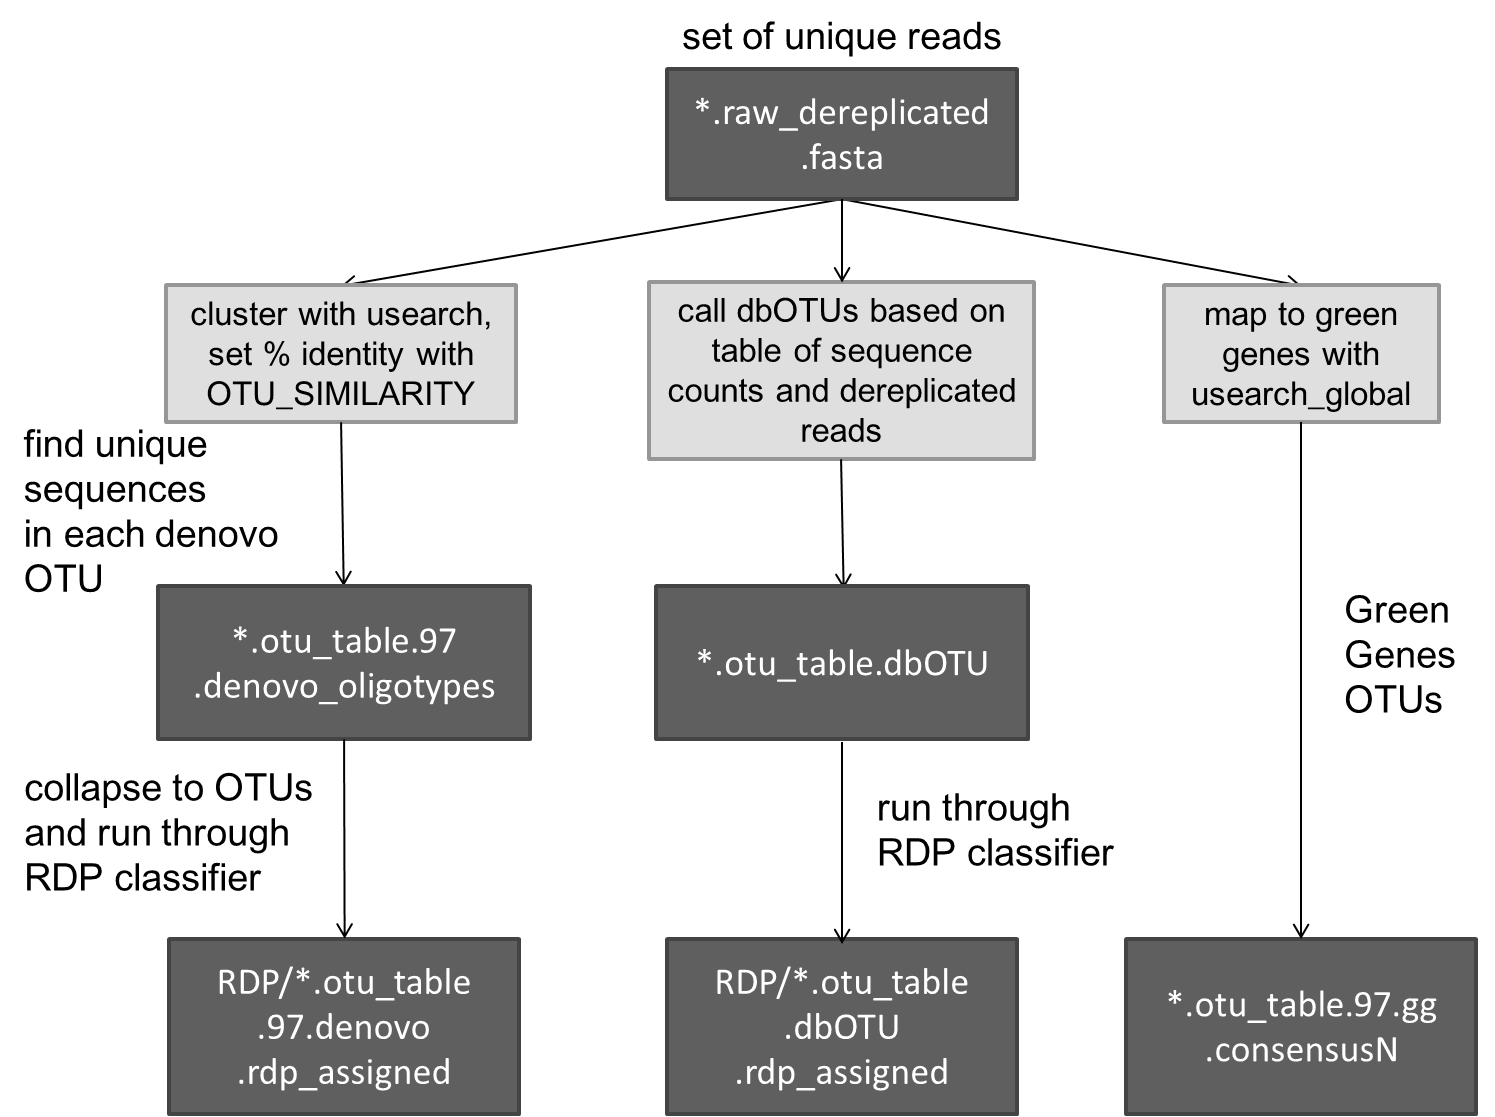
\includegraphics[width=0.8\textwidth]{figs/OTU_calling.png}
\caption{Schematic of OTU calling pipeline.}
\end{figure}


\subsubsection{\textit{de novo} OTU tables}
The dereplicated reads are clustered to within the specified sequence similarity percentage cut-off ({\tt OTU\_SIMILARITY}, default: 97) using {\tt usearch}.  Individual reads are assigned either as the OTU centroid or as a match. Centroids are labeled as 'OTU\_ID.0' and matches count from 'OTU\_ID.1' onwards.  These are separate oligotypes within the OTU 'OTU\_ID'. All oligotype counts are then collapsed to their respective OTU, resulting in a fully \textit{de novo} OTU table which can be found in the filename {\tt datasetID.otu\_table.*.denovo} where '{\tt *}' gets replaced by the OTU similarity cut-off.

\subsubsection{Closed-reference OTU table}
There are two types of database-referencing that are outputed from the pipeline by default.  The first is assignments from the Ribosomal Database Project (RDP), which returns probabilistic assignments.  The default probability cut-off below which an assignment is labeled as unidentified at a given taxonomic level is 0.5, but this can be set using a summary file parameter {\tt RDP\_CUTOFF}.  This OTU table can be found in the results sub-folder called 'RDP'.

The dereplicated reads are also aligned to a standard database (GreenGenes in the case of 16S sequences and UNITE in the case of ITS sequences).  In the case of GreenGenes, the database is determined based on the specified OTU similarity cut-off: e.g. {\tt 97\_otus.fasta} for {\tt OTU\_SIMILARITY} set to 97).  The alignment is performed using {\tt usearch}, and considers the top 10 hits.  Consensus assignments are then produced for the top 1, top 3, top 5 and top 10 hits (where a taxonomic level is only assigned a latin name if the top N hits from GreenGenes agree), and the corresponding OTU tables are output.  Thus, the OTU table called {\tt datasetID.otu\_table.*.gg.consensus10} contains latin names which are formed from a minimum consensus of the top 10 hits for each taxonomic level, where '{\tt *}' gets replaced by the OTU similarity cut-off.  Levels are left unidentified (e.g. '{\tt s\_\_}') if the consensus requirement is not met.  

Note that the database referencing process is one of the slower steps in the pipeline, so if you only care about RDP, you can skip the GreenGenes assignments steps by setting the parameter {\tt GG\_ALIGN} to {\tt False} in the summary file.  Similarly, for ITS sequences, you can skip the UNITE assignments steps by setting the parameter {\tt UNITE\_ALIGN} to {\tt False}.

\subsubsection{Open-reference OTU table}
{\tt DEPRECATED:} The pipeline no longer produces open-reference OTUs. 

If any reads in the dereplicated sequences do not align to GreenGenes/UNITE to within the specified similarity cut-off, they are clustered with the desired similarity cut-off using {\tt usearch}, and appended to the GreenGenes/UNITE closed-reference table to produce a full, open-reference OTU table (which combines GreenGenes-referenced and \textit{de novo} OTUs) at the desired similarity cut-off, with filename {\tt datasetID.otu\_table.gg.*.open\_ref}.

\subsubsection{Oligotypes}
The OTU calling process automatically assigns separate IDs to unique sequences within OTUs (termed 'oligotypes' by some).  These offer a greater level of granularity.  For example, if sequences A, B and C are all the same OTU, called OTU1 (and the centroid is sequence A), these would be relabeled 'OTU1.0', 'OTU1.1' and 'OTU1.2'. Note that
these unique `oligotypes' are generated by any fancy information-based algorithms -
they are simply the unique sequences within each OTU.

There is currently one such table output: the full \textit{de novo} oligotype table (where sequences are labeled according to a fully \textit{de novo} OTU clustering process) - \\{\tt myDataset.otu\_table.N.denovo\_oligotypes}

\section{Source code - Python modules}
The following code can all be in \texttt{/home/ubuntu/scripts}. Some of these scripts
are used by the pipeline, others are not currently incorporated but may still prove
useful to your 16S-related work.

\subsection{Modules}
\begin{itemize}
  \item {\tt Formatting.py} - Module to house miscellaneous formatting methods, e.g. conversion from classic dense format to BIOM format, OTU table transposition, etc.
	\item {\tt QualityControl.py} - Methods for quality control diagnostics on a dataset.
	\item {\tt preprocessing\_16S.py} - Methods and wrappers for raw 16S sequence data processing.
	\item {\tt Taxonomy.py} - Methods for taxonomy-related feature extraction and analytics.  Includes functions for things like:
		-adding latin names to a GreenGenes-referenced OTU table
		-collapsing abundances at different taxonomic levels
	\item {\tt Phylogeny.py} - Methods for phylogenetic feature extraction, e.g. left/right (LR) abundance ratios at each node of a phylogenetic tree.
	\item {\tt Analytics.py} - Generic statistical analysis tools, e.g. Wilcoxon tests across all available taxa.
	\item {\tt Regressions.py} - Performs different types of regressions \textit{en masse}.
	\item {\tt FileManipulations.py} - Methods for reading and moving around raw data files.
\end{itemize}

\subsection{Scripts and routines}
\begin{itemize}
	\item {\tt Master.py} - Master script that calls relevant processing pipelines, e.g. {\tt raw2otu.py}.
	\item {\tt raw2otu.py} - Pipeline for converting raw 16S FASTQ sequence files to OTU tables.  Handles parallelization requirements in these processing steps automatically.  Takes as input a directory that contains a summary file and the raw data.
\end{itemize}

\section{Troubleshooting}
Standard error ({\tt stderr}) and standard out ({\tt stdout}) are directed to the directory {\tt /home/ubuntu/logs}.  Errors will appear in the {\tt stderr} file for the corresponding datasets.  There may also be useful errors in the \texttt{stderr\_master.log}
and \texttt{stdout\_master.log} files that are created in the directory
from which you ran the \texttt{python Master.py} call.
In addition, file outputs from each step of the pipeline can be found in {\tt /home/ubuntu/proc/datasetID\_proc\_16S}, which can help to diagnose errors.  Common sources of errors or difficulties include:

\begin{itemize}
\item Bad formatting of the summary, barcodes, or primers file.  There should be no white spaces, and columns should be tab-delimited.  If you created the file in Excel, it may have carriage return or other non-linux formatting characters that introduce difficulties.  Safest is to go from a previous summary file template, or to create it manually.
\item Typos in a 16S attribute key-value pair in the summary file.
\item Incorrect ASCII encoding specified.  Check whether 33 or 64 using {\tt usearch8 -fastq\_chars yourFASTQfile.fastq}.  Default is 33, so if left unspecified and the file is ASCII base 64, quality trimming will fail.
\item For ITS sequences, the RDP classifier often runs out of RAM when loading the UNITE database.  This is usually what happened if you find {\tt RDP\_classification.txt} to be empty in the relevant folder in {\tt /home/ubuntu/proc}.  If you rerun the pipeline several times, have checked everything else and keep encountering this problem, you may need a node with more RAM to do your processing.
\item If you specify a file containing a list of FASTQ/FASTA files for the raw reads, make sure the file paths are relative to the directory hosting the summary file.
\end{itemize}

\section{Appendix}
\subsubsection{List of 16S and ITS attributes}\label{sec:summarytable}
\begin{center}
\begin{longtable}{| c | c |}
    \hline
      \textbf{Attribute} & \textbf{Description} \\
      \hline
      {\tt RAW\_FASTQ\_FILE} & Raw FASTQ file name/path within the dataset directory \\
      \hline
      {\tt RAW\_FASTA\_FILE} & Raw FASTA file name/path if raw data is in FASTA format \\
      \hline
      {\tt RAW\_FASTQ\_FILES}
       & For demultiplexed datasets where samples are separated \\
       & into separate FASTQ files.  Filename of two column file \\
       & containing FASTQ filenames in first column and sample IDs \\
       & in the second column. \\
       \hline
      {\tt RAW\_FASTA\_FILES} 
       & For demultiplexed datasets where samples are separated \\
       & into separate FASTA files.  Filename of two column file \\
       & containing FASTA filenames in first column and sample IDs \\
       & in the second column. \\
       \hline
      {\tt ASCII\_ENCODING} & ASCII quality encoding in FASTQ.  Supports either \\
       & 'ASCII\_BASE\_33'  or 'ASCII\_BASE\_64'.  Set to 33 if unspecified. \\
       \hline
      {\tt PRIMERS\_FILE} & Filename/path to primers file. \\
       & {\tt required}: If primers have already been removed, specify 'None'. \\
       \hline
      {\tt BARCODES\_MAP} & Filename/path to barcodes map file. \\
       & Tab-delimited file contains sampleIDs in first column \\
       & and barcode sequences in second column. \\
       & {\tt required}: If barcodes have already been removed, specify 'None'. \\
       \hline
      {\tt BARCODES\_MODE} & '1' = barcodes in sequence ID, \\
       &  '2' = barcodes in sequences themselves. \\
       & Required if {\tt BARCODES\_MAP} is not None. \\
       \hline
       {\tt BARCODES\_SEPARATOR} & Separator character.  See description in Case 2 below. \\
       \hline
       {\tt METADATA\_FILE} & Filename/path to metadata file. \\
       \hline
       {\tt MERGE\_PAIRS} & If need to merge paired-end reads, set to "True". \\
       \hline
       {\tt FWD\_SUFFIX} & Filename suffix of files with forward reads. \\
       & Should include filename extension. If not specified, defaults to {\tt \_1.fastq}\\
       \hline
       {\tt REV\_SUFFIX} & Filename suffix of files with reverse reads. \\
       & Should include filename extension. If not specified, defaults to {\tt \_2.fastq}\\
       \hline
       {\tt PROCESSED} & True/False flag for whether data have already been processed. \\
        & {\tt required}: Set to 'False' for processing to proceed. \\
        \hline
        {\tt TRIM\_LENGTH} & Length to which all sequences should be trimmed.  \\
        & Defaults to 101 if unspecified. \\
        \hline
        {\tt QUALITY\_TRIM} & Minimum quality score allowed.  \\
        & Sequences are truncated at the first base having quality \\
        & score less than {\tt value}.  Defaults to 25 if unspecified. \\
        & If set to {\tt None}, no quality filtering or trimming will be performed. \\
        & If both {\tt QUALITY\_TRIM} and {\tt MAX\_ERRORS} are included in summary file, \\
        & {\tt MAX\_ERRORS} will be ignored (even if {\tt QUALITY\_TRIM = None}). \\
        \hline
		{\tt MAX\_ERRORS} & Maximum expected errors allowed. \\
		& After length trimming, sequences with more than {\tt MAX\_ERRORS} \\
		& expected errors are discarded. If not specified or if a {\tt TRIM\_QUALITY} value \\
		& is specified, defaults to quality trimming behavior, above. \\
		\hline
        {\tt MIN\_COUNT} & Minimum sequence count in dereplication across \\
        & all samples.  Defaults to 10 if unspecified (i.e. sequences with fewer than  \\
        & 10 occurrences in the entire dataset will not be considered downstream). \\
        \hline
        {\tt OTU\_SIMILARITY} & Integer specifying the percent similarity desired \\
         &  in OTU clustering.  Defaults to 97 if unspecified. \\
	\hline
	{\tt RDP\_CUTOFF} & Desired probability cut-off for Ribosomal Database Project \\
	& assignments.  Assignments at each taxonomic level will be evaluated and \\
	& those with a lower probability than this cutoff will be \\
	& labeled as unidentified. Defaults to 0.5 if unspecified. \\
	\hline
	{\tt GG\_ALIGN} & Specific to 16S sequences.  True/False flag for whether \\
	& GreenGenes alignments are desired.  Defaults to 'True' if unspecified. \\
	\hline
	{\tt UNITE\_ALIGN} & Specific to ITS sequences.  True/False flag for whether \\
	& UNITE alignments are desired.  Defaults to 'True' if unspecified. \\
	\hline
	{\tt OUTDIR} & Full path to processing directory. Defaults \\
	& to {\tt /home/ubuntu/proc/} if not specified. \\
	\hline
\end{longtable}
\end{center}



\end{document}  